
\lecture{Binomial Random Variables}{binomial-random-variables}
\section{Binomial Random Variables}

\title{Binomial Random Variables}
\subtitle{It is either one or the other}

%\author{Kelly Black}
%\institute{Clarkson University}
\date{25 January 2013}

\begin{frame}
  \titlepage
\end{frame}

\begin{frame}
  \frametitle{Outline}
  \tableofcontents[pausesection,hideothersubsections,sectionstyle=show/hide]
\end{frame}


\subsection{Clicker Quiz}


\iftoggle{clicker}{%
  \begin{frame}
    \frametitle{Clicker Quiz}

    You are going to flip a coin three times. What is the probability of
    getting two tails?

    \vfill

    \begin{tabular}{l@{\hspace{3em}}l@{\hspace{3em}}l@{\hspace{3em}}l}
      A: 1/8 & B: 2/8 & C: 3/8 & D: 4/8
    \end{tabular}

    \vfill
    \vfill
    \vfill


  \end{frame}
}


\begin{frame}
  \frametitle{Four flips}

  You are going to flip a coin four times. What is the probability of
  getting three tails?

    \vfill

\end{frame}


\begin{frame}{Turn It Around}

  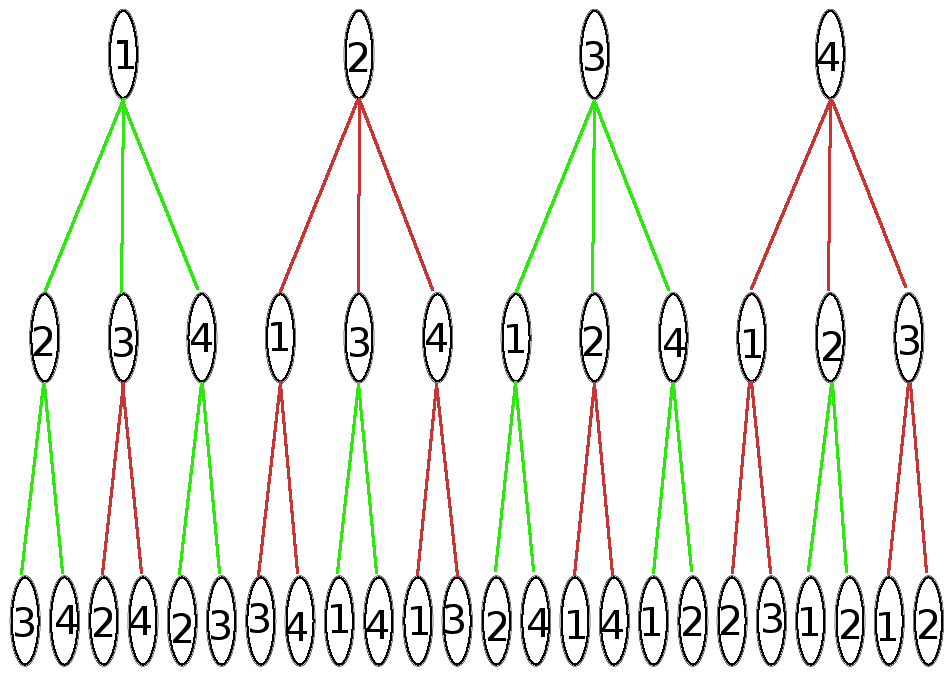
\includegraphics[width=11cm,height=6cm]{img/binomialTree}
  
\end{frame}

\subsection{Binomial Distribution}

\begin{frame}{Binomial Distribution}

  \begin{itemize}
  \item I have $N$ experiments.
  \item Each experiment has only two possible outcomes (Yes/No).
  \item Each experiment has a probability $p$ of a ``yes'' outcome.
  \item Each experiment is independent of the others.
  \end{itemize}

  \vfill

  Question: What is the probability of $k$ ``yes'' outcomes?

  \vfill

  In general we have 
  \begin{eqnarray*}
    \underbrace{
      \rule{.3cm}{.2mm} \hspace{.05cm} 
      \rule{.3cm}{.2mm} \hspace{.05cm} 
      \rule{.3cm}{.2mm} \hspace{.05cm} 
      \rule{.3cm}{.2mm} \hspace{.05cm} 
      \rule{.3cm}{.2mm} \hspace{.05cm} \ldots
      \rule{.3cm}{.2mm} \hspace{.05cm} 
      \rule{.3cm}{.2mm} \hspace{.05cm}}_{\mathrm{n~possible~outcomes}}
    & \rightarrow & 
    \underbrace{
      \rule{.3cm}{.2mm} \hspace{.05cm} 
      \rule{.3cm}{.2mm} \hspace{.05cm} 
      \rule{.3cm}{.2mm} \hspace{.05cm} \ldots
      \rule{.3cm}{.2mm} \hspace{.05cm} 
      \rule{.3cm}{.2mm} \hspace{.05cm}}_{\mathrm{k~Yes}}
    \bigg|
    \underbrace{
      \rule{.3cm}{.2mm} \hspace{.05cm} 
      \rule{.3cm}{.2mm} \hspace{.05cm} 
      \rule{.3cm}{.2mm} \hspace{.05cm} \ldots
      \rule{.3cm}{.2mm} \hspace{.05cm} 
      \rule{.3cm}{.2mm} \hspace{.05cm}}_{\mathrm{N-k~No}}
  \end{eqnarray*}



  
\end{frame}

\begin{frame}{Binomial Distribution}

  In general we have 
  \begin{eqnarray*}
    \underbrace{
      \rule{.3cm}{.2mm} \hspace{.05cm} 
      \rule{.3cm}{.2mm} \hspace{.05cm} 
      \rule{.3cm}{.2mm} \hspace{.05cm} 
      \rule{.3cm}{.2mm} \hspace{.05cm} 
      \rule{.3cm}{.2mm} \hspace{.05cm} \ldots
      \rule{.3cm}{.2mm} \hspace{.05cm} 
      \rule{.3cm}{.2mm} \hspace{.05cm}}_{\mathrm{n~possible~outcomes}}
    & \rightarrow & 
    \underbrace{
      \rule{.3cm}{.2mm} \hspace{.05cm} 
      \rule{.3cm}{.2mm} \hspace{.05cm} 
      \rule{.3cm}{.2mm} \hspace{.05cm} \ldots
      \rule{.3cm}{.2mm} \hspace{.05cm} 
      \rule{.3cm}{.2mm} \hspace{.05cm}}_{\mathrm{k~Yes}}
    \bigg|
    \underbrace{
      \rule{.3cm}{.2mm} \hspace{.05cm} 
      \rule{.3cm}{.2mm} \hspace{.05cm} 
      \rule{.3cm}{.2mm} \hspace{.05cm} \ldots
      \rule{.3cm}{.2mm} \hspace{.05cm} 
      \rule{.3cm}{.2mm} \hspace{.05cm}}_{\mathrm{N-k~No}}
  \end{eqnarray*}

  \vfill

  The probability of this particular outcome is $p^k(1-p)^{N-k}$. 

  \vfill

  There are $\prescript{~}{n}{C}_k$ ways to get $k$ ``yes'' results.
  
  \vfill

  \textbf{Binommial Distribution:}\\
  {\color{red}
    The probability of $k$ ``yes'' outcomes is 
    $\prescript{~}{n}{C}_k \cdot p^k (1-p)^{N-k}$.} 

  \vfill

  
\end{frame}



\subsection{Examples}

\begin{frame}
  \frametitle{Example}

  It is estimated that in a given monthly period 55\% of all stocks
  will rise. I pick four stocks at random (with replacement). What is
  the probability that I get exactly one stock that rises?

  \vfill

\end{frame}


\begin{frame}
  \frametitle{Example}

  It is estimated that 2\% of the shirts made at a factory are not
  suitable for sale. You choose 20 shirts at random (with
  replacement). What is the probability that you find exactly three
  unsuitable shirts?

  \vfill

\end{frame}

\iftoggle{clicker}{%
  \begin{frame}{Clicker Quiz}

    A basketball player has a lifetime average of making 70\% of her
    free throws. In a particular game she will attempt seven free
    throws. What is the probability that she will make exactly five free
    throws?

    \vfill

    \begin{tabular}{l@{\hspace{3em}}l@{\hspace{3em}}l@{\hspace{3em}}l}
      A: .015 & B: .105 & C: .32 & D: .64
    \end{tabular}

    \vfill
    \vfill
    \vfill
  
  \end{frame}
}


% LocalWords:  Clarkson pausesection hideallsubsections
